% This is samplepaper.tex, a sample chapter demonstrating the
% LLNCS macro package for Springer Computer Science proceedings;
% Version 2.20 of 2017/10/04
%
\documentclass[runningheads,a4paper]{llncs}
%
\usepackage{graphicx}
\usepackage[latin1]{inputenc}
\usepackage{amsmath, amssymb, amsfonts, dsfont, mathtools}
% Used for displaying a sample figure. If possible, figure files should
% be included in EPS format.
\usepackage{color}
\usepackage{multirow,array}%multicol
\usepackage [ all ]{xy}
\usepackage{pict2e,picture}
\usepackage{epsfig}
\usepackage{xcolor,tikz}
\usetikzlibrary{fit}
\usepackage{verbatim}
\usepackage[ruled,vlined,linesnumbered]{algorithm2e}
\usepackage{array}

\newcommand{\keywords}[1]{\par\addvspace\baselineskip
\noindent\keywordname\enspace\ignorespaces#1}

\usepackage{soul,hyperref}


\newcommand{\K}{\mathbb{K}}
\newcommand{\M}{\mathbb{M}}
\newcommand{\calC}{\mathcal C}
\newcommand{\cM}{\mathcal M}
\newcommand{\up}[1][]{{^{\uparrow_{#1}}}}
\newcommand{\down}[1][]{{^{\downarrow^{#1}}}}
\renewcommand{\emptyset}{\varnothing}
\newcommand{\obotSymbol}{%
	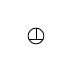
\begin{tikzpicture}[scale=0.1, line width=0.11mm]
		\draw (0,-0.5)--(0,1); \draw (-0.866,-0.5)--(0.866,-0.5);
		\draw (0,0) circle [radius=1];
\end{tikzpicture}}
\newcommand{\obot}{\mathbin{\raisebox{-0pt}{\obotSymbol}}}
\newcommand{\cupbotSymbol}{%
	\begin{tikzpicture}[scale=0.1, line width=0.11mm]
		\draw (0,-0.5) -- (0,1);
		\draw (-0.866,-0.5) -- (0.866,-0.5);
		\node[scale = 1] () at (0,0) {$\cup$};
\end{tikzpicture}}
\newcommand{\cupbot}{\mathbin{\raisebox{-2.5pt}{\cupbotSymbol}}}
\newcommand{\adjoint}{\mathop{\&}\nolimits}
\newcommand{\G}{\text{G}}
\let\oldLcommand\L
\let\L\relax
\def\L{\text{\oldLcommand}}

\newcommand{\editornote}[1]{{\color{red}[#1]}}
\newcounter{editorcommentcounter}
\newcommand{\editorcomment}[2][]{{%
	\normalfont
	\stepcounter{editorcommentcounter}%
	\textsuperscript{\textcolor{red}{(\arabic{editorcommentcounter})}}%
	\marginpar{\footnotesize\textcolor{red}{\arabic{editorcommentcounter}. #2}}%
}}



\newcommand{\cred}[1]{{\color{red} #1}}
\newcommand{\cb}[1]{{\color{blue}#1}}
\newcommand{\cy}[1]{{\color{cyan} #1}}
\newcommand{\cg}[1]{{\color{green!50!black} #1}}
%
\newcommand{\ct}[1]{\cred{\textst{#1}}}
\definecolor{naranjauca}{cmyk}{ 0, 0.6, 1, 0}
%\xdefinecolor{naranjauca}{rgb}{1, 0.45, 0}
\newcommand{\cn}[1]{{\color{naranjauca} #1}}
\def\seealso#1{\mbox{}%
	\marginpar[\raggedleft $\rightarrow$\\ \small \cn{#1}]%
	{\raggedright $\leftarrow$\small \cn{#1}}\ignorespaces}

\def\seealsob#1{\mbox{}%
	\marginpar[\raggedleft $\rightarrow$\\ \small {#1}]%
	{\raggedright $\leftarrow$\small {#1}}\ignorespaces}
% If you use the hyperref package, please uncomment the following line
% to display URLs in blue roman font according to Springer's eBook style:
\renewcommand\UrlFont{\color{blue}\rmfamily}

\begin{document}
	
\mainmatter  % start of an individual contribution

%
\title{\cred{Introducing the notion of bond in the multi-adjoint framework}\thanks{Partially supported by the the 2014-2020 ERDF Operational Programme in collaboration with the State Research Agency (AEI) in project PID2019-108991GB-I00, and with the Department of Economy, Knowledge, Business and University of the Regional Government of Andalusia in project FEDER-UCA18-108612, and by the European Cooperation in Science \& Technology (COST) Action CA17124.}}
%
\titlerunning{}
%Factorization of multi-adjoint contexts based on thresholds}
% If the paper title is too long for the running head, you can set
% an abbreviated paper title here
%
\author{Roberto G. Aragón%\orcidID{0000-0002-8927-5945} 
\and
Jesús Medina%\orcidID{0000-0002-3931-5873} 
\and
Samuel Molina Ruiz%\orcidID{0000-0002-2391-5217}
}
%
\authorrunning{R.G. Aragón, J. Medina, S. Molina}
% First names are abbreviated in the running head.
% If there are more than two authors, 'et al.' is used.
%
\institute{Department of Mathematics, University of Cádiz, Spain
\email{\{roberto.aragon,jesus.medina,samuel.molina\}@uca.es}}
%
\maketitle              % typeset the header of the contribution
% 
\begin{abstract}

	
\keywords{Formal concept analysis, bond, multi-adjoint framework, concept lattice}
\end{abstract}

\section{Introduction}

The ability to process large amounts of data efficiently is essential for extracting useful information from databases. Formal concept analysis (known in short as FCA) has been one of the most widely used and developed mathematical theory for extracting knowledge from relational databases since its introduction in the eighties~\cite{Wille:1982}. The theory deems databases as formal contexts~\cite{GanterW}, which consist of a set of objects, a set of attributes, and a relationship between these sets. FCA tools are capable of manipulating data and extracting relevant information, which is then represented using the algebraic structure of a complete lattice~\cite{?}.  Several extensions of this mathematical theory have been introduced in a fuzzy environment. Among them, the multi-adjoint framework~\cite{TFS:2020-acmr,ar:ins:2015,ins2018:cmr,mor-fss-cmpi} is one of the most flexible and versatile, making it ideal for modeling real-world problems.

Various methods have been developed and utilized in FCA to simplify data processing,%~\cite{bmrd:FCARST:f,Cornejo2017},
such as factoring and aggregating data tables~\cite{COAMfac2024,BELOHLAVEK20103,dubois:2012,KRIDLO22IS,valverdeipmu18art}. These techniques enable the reduction of large tables into smaller tables, known as factors, from which important information can be extracted. Furthermore, these factors can be aggregated without altering the information. 
In particular, we focus on the notion of bond between formal contexts, which was originally defined in the classical setting~\cite{GanterW}  and was extended to the fuzzy framework using residuated lattices~\cite{KridloKO12}.  Bonds permit the aggregation of contexts while preserving the information contained in the concepts generated by each individual context.This work aims to extend the aforementioned notion to the multi-adjoint framework and analyze the conditions that enable obtaining bonds in a simpler manner.



\section{Preliminaries}

In this preliminaries section, we introduce foundational notions related to FCA. Throughout this paper, the notation $A^B$ will be employed to denote maps from $B$ to $A$. Particularly, if $A = \{1, \dots, n\}$ we may use $n^B$ to denote $\{1, \dots, n\}^B$. We now proceed to define what precisely a context is within the setting of FCA.

\begin{definition}

A \emph{context} is a tuple $\cb{\K=}(O, P, R)$ such that $O$ and $P$ are non-empty sets (usually interpreted as objects and properties, respectively) and $R$ is a relation in $O \times P$.

\end{definition}

In addition, the derivation operators $\up \colon 2^O \to 2^P$ and $\down \colon 2^P \to 2^O$ are defined as
\begin{align*}
	X\up &= \{a \in P \mid (x, a) \in R, \text{ for all $x \in X$}\} \\
	A\down &= \{x \in O \mid (x, a) \in R, \text{ for all $a \in A$}\}
\end{align*}
for all $X \subseteq O$ and $A \subseteq P$.
A \emph{concept} is a pair $\langle X, A \rangle$ \cred{where $X$ and $A$ are respectively subsets of objects and properties,}
satisfying that $X\up = A$ and $A\down = X$, \cb{where $X$ is called the \emph{extent} and $A$ is the \emph{intent}}. The set of all the concepts of the context $(O, P, R)$ is denoted by $\calC(O, P, R)$, and with the ordering defined by $\langle X_1, A_1 \rangle \preceq \langle X_2, A_2 \rangle$ if and only if $X_1 \subseteq X_2$ (equivalently $A_2 \subseteq A_1$), for all $\langle X_1, A_1 \rangle, \langle X_2, A_2 \rangle \in \calC(O, P, R)$, forms a complete lattice~\cite{DaveyPriestley} \cb{called  \emph{concept lattice}}. \cred{We will refer to this lattice as the \emph{concept lattice} of the context $(O, P, R)$, and to the objects and properties of a concept as the \emph{extent} and \emph{intent}, respectively.}

% \color{red}
% Additionally, we introduce the notion of a closed relation:

% \begin{definition}
	
% Let $(O, P, R)$ be a context. A subrelation $R' \subseteq R$ is a \emph{closed relation} of the context $(O, P, R)$ if every concept of the context $(O, P, R')$ is also a concept of $(O, P, R)$.

% \end{definition}

% One way to recognize when a relation is closed is given by the following characterization.

% \begin{proposition}\label{prop:characterization-of-bonds}
	
% The closed relations of a context $(O, P, R)$ are precisely those subrelations $R' \subseteq R$ which satisfy the following condition:
% \begin{center}\begin{minipage}{0.9\textwidth}
% 	$(x, a) \in R \setminus R'$ implies $(y, a) \notin R$ for some $y \in O$ with $x\up[R'] \subseteq y\up[R']$ as well as $(x, b) \notin R$ for some $b \in P$ with $p\down[R'] \subseteq b\down[R']$.
% \end{minipage}\end{center}

% \end{proposition}

% The closed relations characterize the complete sublattices of a concept lattice, as shown in the next result.

% \begin{theorem}
	
% If $R'$ is a closed relation of the context $(O, P, R)$, then $\calC(O, P, R')$ is a complete sublattice of $\calC(O, P, R)$, with
% \[
% R' = \bigcup \{X \times A \mid (X, A) \in \calC(O, P, R)\}
% \]
% Inversely, for every complete sublattice $U$ of $\calC(O, P, R)$, the relation
% \[
% R' = \bigcup \{X \times A \mid (X, A) \in U\}
% \]
% is a closed relation of $(O, P, R)$ with $\calC(O, P, R') = U$.

% \end{theorem}

% As explained in the introduction, our focus is on joining a family of contexts. The natural environment for this is the direct, or cartesian, product of concept lattices. We want to study the complete sublattices of this product that preserve the original concept lattices. With this idea in mind, we introduce the notion of a subdirect product.

% \begin{definition}
	
% A \emph{subdirect product} of complete lattices is a complete sublattice of the direct product for which the canonical projections onto the factors is surjective.

% \end{definition}

% In order to work with this notion, we are going to define the direct sum of contexts.

% \begin{definition}
	
% Let $\Lambda$ be an arbitrary set of indices. Given a family $\{\K_i = (O_i, P_i, R_i)\}_{i \in \Lambda}$ of disjoint contexts\footnote{Two contexts $(O_1, P_1, R_1)$ and $(O_2, P_2, R_2)$ are disjoint if $O_1 \cap O_2 = P_1 \cap P_2 = \emptyset$}, we define their \emph{direct sum} as the context $\sum_{i \in \Lambda} \K_i = (O_\Lambda, P_\Lambda, R_\Lambda)$ where\editorcomment{hay un abuso de notación puesto que se usa $\Lambda$, como conjunto de índices y como subíndice (notación). Tendríamos que comentarlo.}
% \[
% O_\Lambda = \bigcup_{i \in \Lambda} O_i, \quad P_\Lambda = \bigcup_{i \in \Lambda} P_i, \quad R_\Lambda = \bigcup_{i \in \Lambda} R_i \cup \bigcup_{j \neq i} (O_j \times P_j).
% \]

% \end{definition}

% The direct sum is a more natural way to work with the direct product of the concept lattices, but it is equivalent thanks to the following theorem.

% \begin{theorem}\label{th:isomorphism-sum-context-lattice---prod-concept-lattice}
	
% The concept lattice of a direct sum of context is isomorphic to the cartesian product of the concept lattice of the factors, that is,
% \[
% \calC ( \sum_{i \in \Lambda} \K_i ) \cong \bigtimes_{i \in \Lambda} \calC(\K_i).
% \]
% The map $\mathfrak C \colon \calC ( \sum_{i \in \Lambda} \K_i ) \to \bigtimes_{i \in \Lambda} \calC(\K_i)$ given by
% \[
% \mathfrak C (X, A) = (X \cap O_i, A \cap P_i)_{i \in \Lambda}, \quad \text{for all $\textstyle(X, A) \in \calC(\sum_{i \in \Lambda} \K_i)$}
% \]
% is a natural isomorphism. Moreover, the canonical projection together with this isomorphism is the map $\pi_i \colon \calC (\sum_{i \in \Lambda} \K_i) \to \calC(\K_i)$ given by 
% \[
% \pi_i(X, A) = (X \cap O_i, A \cap P_i), \quad \text{for all $\textstyle (X, A) \in \calC ( \sum_{i \in \Lambda} \K_i )$}.
% \]

% \end{theorem}

% We end this introduction showing how subdirect products and direct sums relate. This relation lets us use the more natural notion of direct sum in order to join different contexts.

% \begin{proposition}\label{prop:subdirec-products-characterization}
	
% The subdirect product of the concept lattices $\calC(\K_i)$ are one to one with the closed relations $R$ of the sum context $\sum_{i \in \Lambda} \K_i$ with $R \cap (O_i \times P_i) = R_i$ for all $i \in \Lambda$.

% \end{proposition}
% color{black}

\section{Bonds}\label{sec:bonds}

\cb{The aim of this study is to investigate methods for aggregating contexts (factors) and constructing a new context from them. This new context has to preserve the information contained in the factors.}
\cred{Our objective is to study ways of {joining}contexts and constructing a new context from these. We wish for this new context to preserve the information of the factors.} Throughout this section, we will pursue this idea presenting the theory of bonds in the \cred{non-fuzzy}\cb{classical} case and working through an example. \cred{until finally arriving at a remark discussing when the empty set is a bond.} \editornote{No creo que se entienda esto ahora en este punto sin haber definido nada.} In Section~\ref{sec:multi-adjoint}, we will translate these notions into the multi-adjoint framework.

\cb{From now on, we will consider} a family of contexts $\{\K_i = (O_i, P_i, R_i)\}_{i \in \Lambda}$, with $\Lambda$ an \cred{arbitrary}\cb{non-empty} set of indices. 
\cb{We will simply denoted the derivation operators $\up$ and $\down$ in each context $\K_i$ as $\up[i]$ and $\down[i]$, respectively.}
\cred{For every context $\K_i$, we are going to simplify the notation of the derivation operators by dropping the $R$, that is, $\up[R_i]$ and $\down[R_i]$ will simply be denoted as $\up[i]$ and $\down[i]$, respectively. }
Moreover, if $R_{ij} \subseteq O_i \times P_j$ is a relation, we \ct{will} define the mappings $\up[ij] \colon 2^{O_i} \to 2^{P_j}$ and $\down[ij] \colon 2^{P_j} \to 2^{O_i}$ as
\begin{align*}
	X\up[ij] &= \{a \in P_j \mid (x, a) \in R_{ij}, \text{ for all $x \in X$}\} \\
	A\down[ij] &= \{x \in O_i \mid (x, a) \in R_{ij}, \text{ for all $a \in A$}\}
\end{align*}
for all $X \subseteq O_i$ and $A \subseteq P_j$. When we consider $X = \{x\}$ and $A = \{a\}$, we may use the notation $x\up[ij]$ and $a\down[ij]$ instead of $\{x\}\up[ij]$ and $\{a\}\down[ij]$.

Our initial step will involve defining the concept of a bond.

\begin{definition}\label{def:bond}

Given two different contexts $\K_i$ and $\K_j$, a \emph{bond} from $\K_i$ to $\K_j$ is a relation $R_{ij} \subseteq O_i \times P_j$ such that
\begin{itemize}
	\item $x\up[ij]$ is an intent of $\K_j$ for every object $x \in O_i$,
	\item $a\down[ij]$ is an extent of $\K_i$ for every property $a \in P_j$.
\end{itemize}

\end{definition}

A direct consequence of the definition is that for every extent $X$ of $\K_i$ and intent $A$ of $\K_j$, $X\up[ij]$ is an intent of $\K_j$ and $A\down[ij]$ is an extent of $\K_i$. \cred{For instance,
\[
X\up[ij] = \inf \{x\up[ij] \mid x \in X\}
\]
is an intent of $\K_j$.} \editornote{No entiendo esto, parece que se cambiara la definicion del operador no?}

\cb{Now, we will}\ct{Let's} examine this definition more closely through a practical example

\begin{example}\label{ex:crisp-bonds}

Consider two contexts $\K_1 = (O_1, P_1, R_1)$ and $\K_2 = (O_2, P_2, R_2)$ where
\begin{align*}
	O_1 &= \{x_1, x_2\}, & P_1 &= \{a_1, a_2\}, & R_1 &= \{(x_1, a_1), (x_1, a_2), (x_2, a_2)\} \\
	O_2 &= \{x_3, x_4\}, & P_2 &= \{a_3, a_4\}, & R_2 &= \{(x_3, a_3), (x_4, a_4)\}
\end{align*}
A bond can be visualized by placing the two contexts diagonally, one beneath the other, and the bond in the top right corner (a bond $R_{ji}$ from $\K_j$ to $\K_i$ would be placed in the bottom left), as observed in Table~\ref{tab:example-crisp-bonds}. 
Given that the set of objects and the set of properties are always extent and intent of a context, respectively, we are guaranteed that the relation $R_{1\,2}^\top = O_1 \times P_2$ is a bond. Indeed, for any $x \in O_1$ and $a \in P_2$, $x\up[1\,2] = P_2$ is an intent of $\K_2$ and $a\down[1\,2] = O_1$ is an extent of $\K_1$.

\begin{table}[h!]
	\centering
	\begin{tabular}{w{c}{15pt} || w{c}{15pt} | w{c}{15pt} || w{c}{15pt} | w{c}{15pt}}
		& $a_1$ & $a_2$ & $a_3$ & $a_4$ \\\hline\hline
		$x_1$ & $\times$ & $\times$ & $\times$ & $\times$ \\\hline
		$x_2$ & & $\times$ & $\times$ & \\\hline\hline
		$x_3$ & & & $\times$ & \\\hline
		$x_4$ & & & & $\times$\\
	\end{tabular}
	\hspace{1cm}
	\begin{tabular}{w{c}{15pt} || w{c}{15pt} | w{c}{15pt} ||
	w{c}{15pt} | w{c}{15pt}} & $a_1$ & $a_2$ & $a_3$ & $a_4$ \\\hline\hline
	$x_1$ & $\times$ & $\times$ & & \\\hline 
	$x_2$ & & $\times$ &$\times$ & \\\hline\hline 
	$x_3$ & & & $\times$ & \\\hline
	 $x_4$ & & & &	$\times$\\
	 \end{tabular}
	\caption{Tables showing the contexts $\K_1$ and $\K_2$ on the diagonal and the relations $R_{1\,2}^1$ (left table) and $R_{1\,2}^2$ (right table) of the Example~\ref{ex:crisp-bonds} on the top right corner.}
	\label{tab:example-crisp-bonds}
\end{table}

We can usually find other non-trivial bonds, such as
\[
R_{1\,2}^1 = \{(x_1, a_3), (x_1, a_4), (x_2, a_3)\}
\]
For this relation, $x_1\up[1\,2] = \{a_3, a_4\}$ and $x_2\up[1\,2] = \{a_3\}$ are both intents of $\K_2$. The first one because it is the set of properties $P_2$ and the second one because
\[
\{a_3\}\down[2]\up[2] = \{x_3\}\up[2] = \{a_3\}
\]
Likewise, $a_3\down[1\,2] = \{x_1, x_2\}$ and $a_4\down[1\,2] = \{x_1\}$ are extents of $\K_1$, the first one for being the set of objects $O_1$ and the second one because
\[
\{x_1\}\up[1]\down[1] = \{a_1, a_2\}\down[1] = \{x_1\}
\]

However, not all relations in $O_1 \times P_2$ are bonds. Consider for instance the relation $R_{1\,2}^2 = \{(x_2, a_3)\}$. This relation is not a bond because $a_3\down[1\,2] = \{x_2\}$ is not an extent of $\K_1$, that is, 
\[
\{x_2\}\up[1]\down[1] = \{a_2\}\down[1] = \{x_1, x_2\} \neq \{x_2\}
\]


Another interesting case is the empty relation, $R_{1\,2}^\bot = \emptyset$. Because the empty set is neither an extent of $\K_1$ nor an intent of $\K_2$, this relation is not a bond from $\K_1$ to $\K_2$. 

\editornote{A\~nadir ret\'iculos de conceptos. Es necesario aqu\'i?}
% \begin{figure}
% 	\centering
% 	\includegraphics[height = 0.2\textwidth]{im/ex-crisp-K1.png}
% 	\hspace{1cm}
% 	\includegraphics[height = 0.2\textwidth]{im/ex-crisp-K2.png}
% 	\hspace{1cm}
% 	\includegraphics[height = 0.2\textwidth]{im/ex-crisp-R12^top.png}
% 	\hspace{1cm}
% 	\includegraphics[height = 0.2\textwidth]{im/ex-crisp-R12^1.png}
% 	\caption{From left to right: the concept lattices for $\K_1$, $\K_2$, $(O_1, P_2, R_{1\,2}^\top)$, $(O_1, P_2, R_{1\,2}^1)$ and $(O_1, P_2, R_{1\,2}^1 \cup R_{1\,2}^\top)$\editornote{not right.}.}
% \end{figure}
\qed
\end{example}

\begin{remark}\label{rem:bottom-bond-crisp}

Given two contexts $\K_i = (O_i, P_i, R_i)$ and $\K_j = (O_j, P_j, R_j)$, the empty relation is not always a bond from $\K_i$ to $\K_j$ because the empty set \ct{isn't} is not always an extent or intent of a context. However, there are cases where it is actually a bond. If the contexts $\K_i$ and $\K_j$ satisfy that for every object $x \in O_i$ and property $a' \in P_j$, there exists $a \in P_i$ and $x' \in O_j$ such that $(x, a) \notin R_i$ and $(x', a') \notin R_j$, then this guarantees that the empty set is both an extent of $\K_i$ and an intent of $\K_j$ and therefore the empty relation $R_{ij}^\bot$ is a bond from $\K_i$ to $\K_j$.

\end{remark}

\section{Bonds on a multi-adjoint framework}\label{sec:multi-adjoint}

In the previous section, we tackled the non-fuzzy case. If we consider the fuzzy scenario, we need to work with a more general notion of context, where an object can have a non-binary degree of uncertainty as to whether it has a given attribute. In this section, we will \ct{introduce} \cb{recall} the notion of a multi-adjoint framework and concept in order to define \cb{a bond between contexts associated to a multi-adjoint framework}\ct{what a bond could look like in this setting}. \ct{We will present an example and work towards Proposition}~\ref{prop:trivial-multiadjoint-bonds}.

The first thing we need to do is define what we mean by multi-adjoin framework.

\begin{definition}
	
A \emph{multi-adjoint framework} is a tuple $(L_1, L_2, Q, \adjoint_1, \dots, \adjoint_n)$ where $(L_1, \preceq_1)$ and $(L_2, \preceq_2)$ are complete lattices, $(Q, \leq)$ is a poset and $(\adjoint_k, \swarrow^k, \nwarrow_k)$ is an adjoint triple with respect to $L_1$, $L_2$ and $P$, for all $k \in \{1, \dots, n\}$.

\end{definition}

Throughout this section, \cb{a multi-adjoint framework $(L_1, L_2, Q, \adjoint_1, \dots, \adjoint_n)$ will be fixed.}  The definition of a context is defined in the same way as the non-fuzzy, adding a function which designates an adjoint triple to each pair of objects and properties. This notion is formalized in the following definition.

\begin{definition}
	
A \emph{context} is a tuple $\cb{\M=}(O, P, R, \sigma)$, where $O$ is the set of objects, $P$ is the set of properties, $R$ is a $Q$-fuzzy relation $R \colon O \times P \to Q$ and $\sigma \colon O \times P \to \{1, \dots, n\}$ is a mapping which associates a specific adjoint triple in the frame with any element in $O \times P$.

\end{definition}

\ct{Given a multi-adjoint frame,}\editornote{ya se ha fijado arriba} \cb{The extension} of the concept-forming operators \cb{are the mappings} $\up[\sigma] \colon L_1^O \to L_2^P$ and $\down[\sigma] \colon L_2^P \to L_1^O$ \ct{are} defined as:
\begin{align*}
	g\up[\sigma](a) &= \inf \{R(x, a) \swarrow^{\sigma(x, a)} g(x) \mid x \in O\} \\
	f\down[\sigma](x) &= \inf \{R(x, a) \nwarrow_{\sigma(x, a)} f(x) \mid a \in P\}
\end{align*}
for all $g \in L_1^O$, $f \in L_2^P$ and $a \in P$, $x \in O$.
\ct{As usual} In addition, a pair $\langle g, f \rangle$ is called a \emph{multi-adjoint concept} %if $g \in L_1^O$, $f \in L_2^P$ and 
 if equalities $g\up[\sigma] = f$ and $f\down[\sigma] = g$ hold. \cred{The set $g$ is the \emph{extent} of the concept and $f$ is the \emph{intent}.}\editornote{Yo quitaria esto ya que se sobreentiende de lo que es un concepto no? Y meteria la notacion de reticulo de conceptos multiadjuntos como $\cM$}
 
 \cb{
 \begin{definition}\label{fuzzy-attribute}
For each $a\in P$, the fuzzy subsets of attributes $\phi_{a,x}\in L_1^P$ defined, for all $x\in L_1$, as
$$ \phi_{a,x}(a') = \begin{cases}
 x& \hbox{if } a' = a\\
 \bot_1 &\hbox{if } a'\neq a
\end{cases}
$$
will be called \emph{fuzzy-attributes}.
\end{definition}
Analogously, the fuzzy-objects are defined in the same way.
}

Hereon, $\{\M_i = (O_i, P_i, R_i, \sigma_i)\}_{i \in \Lambda}$ will be a family of context of the frame. Given a $Q$-fuzzy relation $R_{ij}$ in $O_i \times P_j$ and $\sigma_{ij} \colon O_i \times P_j \to \{1, \dots, n\}$, we will define the mappings $\up[ij] \colon L_2^{O_i} \to L_1^{P_j}$ and $\down[ij] \colon L_1^{P_j} \to L_2^{O_i}$ as
\begin{align*}
	g\up[ij](a) &= \inf \{R_{ij}(x, a) \swarrow^{\sigma_{ij}(x,a)} g(x) \mid x \in O_i\} \\
	f\down[ij](x) &= \inf \{R_{ij}(x, a) \nwarrow_{\sigma_{ij}(x,a)} f(a) \mid a \in P_j\}
\end{align*}
for each $g \in L_2^{O_i}$, $f \in L_1^{P_j}$ and $a \in P_j$, $x \in O_i$.

In Definition~\ref{def:bond}, we described a bond from $\K_i$ to $\K_j$ as a relation $R_{ij}$ in $O_i \times P_j$, which can also be interpreted as a \ct{whole}\cb{new} context $(O_i, P_j, R_{ij})$. This point of view is fundamental in the definition of a bond in a multi-adjoint framework.

\begin{definition}
	
Given two different contexts $\K_i$ and $\K_j$, a \emph{ multi-adjoint bond}\editorcomment{maneter el ``multi-adjoint'?'} from $\M_i$ to $\M_j$ is a context $\M_{ij} = (O_i, P_j, R_{ij}, \sigma_{ij})$ such that $R_{ij} \subseteq O_i \times P_j$ and $\sigma_{ij} \colon O_i \times P_j \to \{1, \dots, n\}$ satisfying that
\begin{itemize}
	\item $\phi_{x,t}\up[ij]$ is an intent of $\M_j$ for every object $x \in O_i$,
	\item $\phi_{a,s}\down[ij]$ is an extent of $\M_i$ for every property $a \in P_j$,
\end{itemize}
where $s \in L_1$ and $t \in L_2$.

\end{definition}

Notice that from the results in~\cite{GanterW}, given a bond $\M_{ij}$ from $\M_i$ to $\M_j$ and an extent $X$ of $\M_{ij}$, we have that 
\[
X = \inf \{\phi_{a, s}\down[ij] \mid X \subseteq \phi_{a, s}\down[ij], \ a \in P_i, s \in L_1\}
\]
\cred{Mismo comentario que antes, utilizar la notacion de $g$ en lugar de $X$ y tendriamos que definir los fuzzy-attributes no? La a\~nado arriba en azul}
As a consequence, $X$ is an extent of $\M_i$. Dually we can show that all the intents of $\M_{ij}$ are intents of $\M_j$.

\begin{example}\label{ex:multiadjoint-bonds}

Consider the multi-adjoint framework $([0, 1]_4, [0, 1]_4, [0, 1]_4, \adjoint^*_\G, \adjoint^*_\L)$ and the contexts $\M_1 = (O_1, P_1, R_1, \sigma_1)$ and $\M_2 = (O_2, P_2, R_2, \sigma_2)$, where the relations are defined in Table~\ref{tab:example1-multiadjoint-bonds-R1-R2}. and $\sigma_1(x, a) = \adjoint^*_\G$, for all $(x, a) \in O_1 \times P_1$ and $\sigma_2(x', a') = \adjoint^*_\L$, for all $(x', a') \in O_2 \times P_2$.
\begin{table}[h]
	\centering
	\vspace{-0.5cm}
	\begin{minipage}{0.25\textwidth}
	\begin{tabular}{w{c}{20pt} || w{c}{20pt} | w{c}{20pt}}
		$R_1$ & $a_1$ & $a_2$ \\\hline\hline
		$x_1$ & $0.5$ & $0.75$ \\\hline
		$x_2$ & $0.25$ & $1$
	\end{tabular}
	\end{minipage}
	\begin{minipage}{0.2\textwidth}
		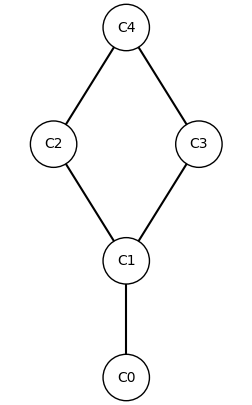
\includegraphics[scale = 0.3]{im/ex-ma2-R1.png}
	\end{minipage}
	% \hspace{1cm}
	\begin{minipage}{0.25\textwidth}
	\begin{tabular}{w{c}{20pt} || w{c}{20pt} | w{c}{20pt}}
		$R_2$ & $a_3$ & $a_4$ \\\hline\hline
		$x_3$ & $1$ & $0.75$ \\\hline
		$x_4$ & $0.75$ & $1$
	\end{tabular}
	\end{minipage}
	\begin{minipage}{0.2\textwidth}
		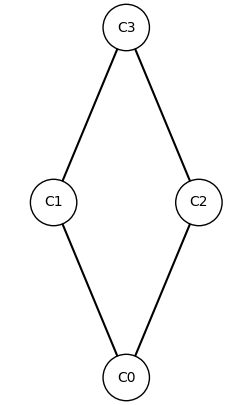
\includegraphics[scale = 0.3]{im/ex-ma2-R2.png}
	\end{minipage}
	\caption{The relations $R_1$ and $R_2$ of the contexts $\M_1$ and $\M_2$ in Example~\ref{ex:multiadjoint-bonds} together with their associated concept lattices.}
	\label{tab:example1-multiadjoint-bonds-R1-R2}
	\vspace{-0.5cm}
\end{table}

Similar to Example~\ref{ex:crisp-bonds}, the relation $R_{1\,2}^\top \equiv 1$ together with any map $\sigma_{1\,2} \colon O_1 \times P_2 \to \{\adjoint^*_\G, \adjoint^*_\L\}$ defines a bond $\M_{1\,2}^\top = (O_1, P_2, R_{1\,2}^\top, \sigma_{1\,2})$ from $\M_1$ to $\M_2$ because $g_\top \colon O_1 \to [0,1]_4$ defined by $g_\top(x) = 1$ for all $x \in O_1$ is an extent of $\M_1$ and $f_\top \colon P_2 \to [0, 1]_4$ defined by $f_\top(a) = 1$ for all $a \in P_2$ is an intent of $\M_2$. There is only one other non-isomorphic\footnote{For every map $\sigma_{1\,2} \colon O_1 \times P_2 \to \{\adjoint^*_\G, \adjoint^*_\L\}$, the contexts $(O_1, P_2, R_{1\,2}, \sigma_{1\,2})$ are all isomorphic in the sense that their concept lattices are the same.} bond from $\M_1$ to $\M_2$ in this example: the bond defined by the relation $R_{1\,2}$ on the second table of Table~\ref{tab:example1-multiadjoint-bonds-R12s}.
\begin{table}[h]
	\centering
	\vspace{-0.5cm}
	\begin{tabular}{w{c}{20pt} || w{c}{20pt} | w{c}{20pt} || w{c}{20pt} | w{c}{20pt}}
		& $a_1$ & $a_2$ & $a_3$ & $a_4$ \\\hline\hline
		$x_1$ & $0.5$ & $0.75$ & $1$ & $1$ \\\hline
		$x_2$ & $0.25$ & $1$ & $1$ & $1$ \\\hline\hline
		$x_3$ & $1$ & $1$ & $1$ & $0.75$ \\\hline
		$x_4$ & $1$ & $1$ & $0.75$ & $1$
	\end{tabular}
	\begin{tikzpicture}[overlay, remember picture]
		\draw[black, ultra thick] (-1.73,-0.12) rectangle (-0.11,0.68);
		\node[right] () at (-0.11,0.28) {$R_{1\,2}^\top$};
		% \draw (-1.73,-0.12) circle (0.02);
		% \draw (-0.11,0.68) circle (0.02);
	\end{tikzpicture}
	\hspace{1cm}
	\begin{tabular}{w{c}{20pt} || w{c}{20pt} | w{c}{20pt} || w{c}{20pt} | w{c}{20pt}}
		& $a_1$ & $a_2$ & $a_3$ & $a_4$ \\\hline\hline
		$x_1$ & $0.5$ & $0.75$ & $1$ & $0.75$ \\\hline
		$x_2$ & $0.25$ & $1$ & $1$ & $1$ \\\hline\hline
		$x_3$ & $1$ & $1$ & $1$ & $0.75$ \\\hline
		$x_4$ & $1$ & $1$ & $0.75$ & $1$
	\end{tabular}
	\begin{tikzpicture}[overlay, remember picture]
		\draw[black, ultra thick] (-1.73,-0.12) rectangle (-0.11,0.68);
		\node[right] () at (-0.11,0.28) {$R_{1\,2}$};
		% \draw (-1.73,-0.12) circle (0.02);
		% \draw (-0.11,0.68) circle (0.02);
	\end{tikzpicture}
	\hspace{1cm}
	\begin{tabular}{w{c}{20pt} || w{c}{20pt} | w{c}{20pt} || w{c}{20pt} | w{c}{20pt}}
		& $a_1$ & $a_2$ & $a_3$ & $a_4$ \\\hline\hline
		$x_1$ & $0.5$ & $0.75$ & $0$ & $0$ \\\hline
		$x_2$ & $0.25$ & $1$ & $0$ & $0$ \\\hline\hline
		$x_3$ & $0$ & $0$ & $1$ & $0.75$ \\\hline
		$x_4$ & $0$ & $0$ & $0.75$ & $1$
	\end{tabular}
	\begin{tikzpicture}[overlay, remember picture]
		\draw[black, ultra thick] (-1.73,-0.12) rectangle (-0.11,0.68);
		\node[right] () at (-0.11,0.28) {$R_{1\,2}^\bot$};
		% \draw (-1.73,-0.12) circle (0.02);
		% \draw (-0.11,0.68) circle (0.02);
	\end{tikzpicture}
	\caption{The relations of the contexts $\M_1$ and $\M_2$ of Example~\ref{ex:multiadjoint-bonds} shown in the diagonal and the relations of the bonds $\M_{1\,2}^\top$ (top left), $\M_{1\,2}$ (top right) and $\M_{1\,2}^\bot$ (bottom) on the upper right corners.}
	\label{tab:example1-multiadjoint-bonds-R12s}
	\vspace{-0.5cm}
\end{table}

Consider now the empty relation $R_{1\,2}^\bot \equiv 0$ and any map $\sigma_{1\,2} \colon O_1 \times P_2 \to \{\adjoint^*_\G, \adjoint^*_\L\}$.
\begin{itemize}
	\item For any $x_i \in O_1$ and $t \in [0, 1]_4$, 
	\begin{align*}
	\phi_{x_i, t}\up[1\,2](a) &= \inf \{R_{1\,2}^\bot \swarrow^{\sigma_{1\,2}(x, a)} \phi(x_i, t) (x) \mid x \in O_1\} \\
	&= \inf \{0 \swarrow^{\sigma_{1\,2}(x, a)} \phi(x_i, t) (x) \mid x \in O_1\} \\
	&= 0
	\end{align*}
	Therefore, $\phi_{x, t}\up[1\,2] \equiv 0$. This fuzzy set will be an intent of $\K_2$ only if $g_\top \colon O_2 \to [0, 1]_L$, $g_\top \equiv 1$, satisfies $g_\top\up[2] \equiv 0$. In this example we have $g_\top\up[2](a_3) = 0.75$ and $g_\top\up[2](a_4) = 0.75$. Hence, the context $\M_{1\,2}^\bot = (O_1, P_2, R_{1\,2}^\bot, \sigma_{1\,2})$ is not a bond from $\M_1$ to $\M_2$.
	\item Dually we have
	\begin{align*}
	\phi_{a_j, s}\down[1\,2](x) &= \inf \{R_{1\,2}^\bot \nwarrow_{\sigma_{1\,2}(x, a)} \phi(a_j, s) (a) \mid a \in P_2\} \\
	&= \inf \{0 \nwarrow_{\sigma_{1\,2}(x, a)} \phi(a_j, s) (x) \mid a \in P_2\} \\
	&= 0
	\end{align*}
	for any $a_j \in P_2$ and $s \in [0, 1]_4$. One could also make the case that for $\M_{1\,2}^\bot$ to qualify as a bond from $\M_1$ to $\M_2$, it is necessary for $\phi_{a, s}\down[1\,2] \equiv 0$ to serve as an extent of $\K_1$. Considering that $f_\top\down[1](x_1) = 0.5$ and $f_\top\down[1](x_2) = 0.25$, with $f_\top \colon P_1 \to [0, 1]_4$ defined as $f_\top \equiv 1$, it follows that $\phi_{a, s}\down[1\,2]$ does not fulfill the role of an intent of $\K_1$. Consequently, we deduce once more that $\M_{1\,2}^\bot$ is not a bond between $\M_1$ and $\M_2$.
\end{itemize}
It is interesting to note that the third concept lattice in \ref{fig:example1-multiadjoint-bonds-concept-lattices} is the \editornote{suma disjunta}\editorcomment{No recuerdo cómo se llamaba a este tipo de unión de retículos. Dados dos retículos, se pueden unir colocándolos uno al lado del otro y uniendo el bottom element de cada uno con un nuevo bottom element, y haciendo lo mismo con los top elements. Roberto ha hecho referencia a este tipo de union en varias ocasiones. Si queremos hablar de esto, deberíamos introducirlo en la sección de preliminares, no?} of the concept lattices $\calC(\M_1)$ and $\calC(\M_2)$.

\begin{figure}
	\centering
	\begin{minipage}{0.3\textwidth}
		\centering
		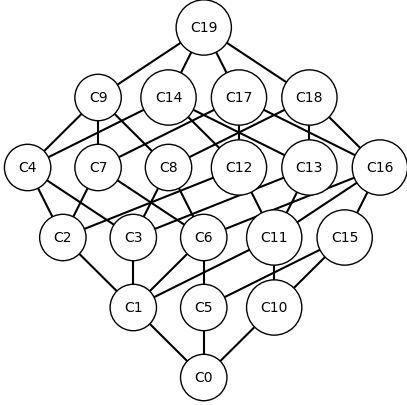
\includegraphics[width = \textwidth]{im/ex-ma2-R1+R2 (top).png}
	\end{minipage}
	\begin{minipage}{0.3\textwidth}
		\centering
		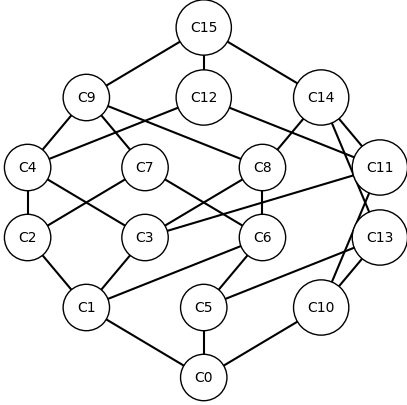
\includegraphics[width = \textwidth]{im/ex-ma2-R1+R2 (other).png}
	\end{minipage}
	\begin{minipage}{0.3\textwidth}
		\centering
		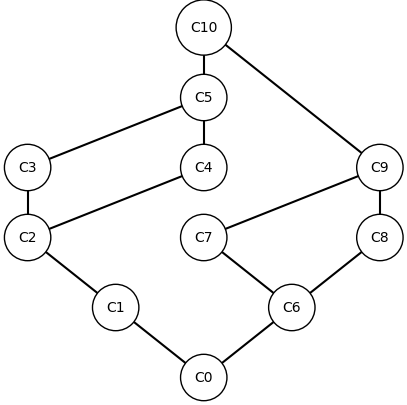
\includegraphics[width = \textwidth]{im/ex-ma2-R1+R2 (bot).png}
	\end{minipage}
	\caption{The concept lattices for the three contexts shown in Table~\ref{tab:example1-multiadjoint-bonds-R12s}, in order.}
	\label{fig:example1-multiadjoint-bonds-concept-lattices}
\end{figure}

\end{example}

Going forward, we will presume that $Q$ constitutes a lattice and that every lattice under consideration is equipped with top and bottom elements, $\top_1$ and $\bot_1$ for $L_1$, $\top_2$ and $\bot_2$ for $L_2$, and $\top_3$ and $\bot_3$ for $Q$, respectively. In this setting we can study the relations $R_{ij}^\top$ and $R_{ij}^\bot$.

As in the classical case (Remark~\ref{rem:bottom-bond-crisp}), the relation $R_{1\,2}^\bot \equiv \bot_3$ does not always define a bond from a context $\M_i$ to another context $\M_j$. This was the case with Example~\ref{ex:multiadjoint-bonds}. In Remark~\ref{rem:bottom-bond-crisp} we showed a characterization of when the non-fuzzy relation $R_{1\,2}^\bot$ was indeed a bond, and we can show a similar property for multi-adjoint bonds. The key idea behind the next proposition is that for $\M_{ij}^\bot$ to be a bond from $\M_i$ to $\M_j$, the sets $g_\bot \colon O_i \to L_1$ and $f_\bot \colon P_j \to L_2$ defined by $g_\bot \equiv \bot_1$ and $f_\bot \equiv \bot_2$ have to be extent of $\M_1$ and intent of $\M_2$, respectively.

\begin{proposition}\label{prop:trivial-multiadjoint-bonds}
	
Consider a multi-adjoint framework $(L_1, L_2, Q, \adjoint_1, \dots, \adjoint_n)$ and two different contexts $\M_i$ and $\M_j$. Given any map $\sigma_{ij} \colon O_i \times P_j \to \{1, \dots, n\}$ and the relation
\[
R_{ij}^\top(x, a) = \top_3, \quad \text{for all $(x, a) \in O_i \times P_j$}
\]
the context $\M_{ij}^\top = (O_i, P_j, R_{ij}^\top, \sigma_{ij})$ is a bond. Moreover,
% if for every $x \in O_i$ and $a' \in P_j$ there exists $a \in P_i$ and $x' \in O_j$ such that $R_i(x, a) = R_j(x', a') = \bot_3$,
if for every row in $R_i$ and column in $R_j$ there is at least one bottom element,
then the context $\M_{ij}^\bot = (O_i, P_j, R_{ij}^\bot, \sigma_{ij})$, where
\[
R_{ij}^\bot(x, a) = \bot, \quad \text{for all $(x, a) \in O_i \times P_j$}
\]
is a bond.

\end{proposition}

\begin{remark}
	
The previous result is a characterization, hence if there is a row in $R_i$ or a column in $R_j$ with no bottom elements, the context $\M_{ij}^\bot$ will not be a bond from $\M_i$ to $\M_j$.

\end{remark}

A particular case of this occurs when both $\M_i$ and $\M_j$ are normalized contexts.

\cb{
\begin{definition}\label{def:normalized-multiadjoint-context}
When $Q$ is bounded with the top element $\top_3$ and the bottom element $\bot_3$, that is, $(Q,\leq,\bot_3,\top_3)$, a context $\M$ will be called \emph{normalized} if there are no rows or columns of the  $Q$-fuzzy relation with all values equal to bottom or with all values different from bottom.
%A context $\M = (O, P, R, \sigma)$ is said to be \emph{normalized} if for every object $x \in O$ and property $a' \in P$, there exists $a, b \in P$ and $x', y' \in O$ such that
%\[
%R(x, a) = \bot, \quad R(x, b) = \top, \quad R(x', a') = \bot, \quad R(y', a') = \top
%\]
\end{definition}
}

\begin{corollary}

If the contexts $\M_i$ and $\M_j$ are normalized in the sense of Definition~\ref{def:normalized-multiadjoint-context}, then for any mappings $\sigma_{ij} \colon O_i \times P_j \to \{1, \dots, n\}$ and $\sigma_{ji} \colon O_j \times P_i \to \{1, \dots, n\}$, the contexts $\M_{ij}^\bot = (O_i, P_j, R_{ij}^\bot, \sigma_{ij})$ and $\M_{ji}^\bot = (O_j, P_i, R_{ji}^\bot, \sigma_{ji})$ are bonds from $\M_i$ to $\M_j$ ahd from $\M_j$ to $\M_i$, respectively.

\end{corollary}

\begin{example}\label{ex:multiadjoint-bonds-2}
	
We will continue working with the multi-adjoint framework defined in Example~\ref{ex:multiadjoint-bonds}. Consider the contexts $\M_3 = (O_3, P_3, R_3, \sigma_3)$ and $\M_4 = (O_4, P_4, R_4, \sigma_4)$, where $R_3$ and $R_4$ are defined by the Table~\ref{tab:example2-multiadjoint-bonds-R3-R4}, $\sigma_3(x, a) = \adjoint^*_\G$ for all $(x, a) \in O_3 \times P_3$ and $\sigma_4(x', a') = \adjoint^*_\L$ for all $(x', a') \in O_4 \times P_4$.
\begin{table}[h]
	\centering
	\vspace{-0.5cm}
	\begin{minipage}{0.25\textwidth}
	\begin{tabular}{w{c}{20pt} || w{c}{20pt} | w{c}{20pt}}
		$R_3$ & $a_1$ & $a_2$ \\\hline\hline
		$x_1$ & $0.75$ & $0$ \\\hline
		$x_2$ & $0.25$ & $0$
	\end{tabular}
	\end{minipage}
	\begin{minipage}{0.2\textwidth}
		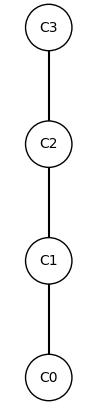
\includegraphics[scale = 0.3]{im/ex-ma2-R3.png}
	\end{minipage}
	% \hspace{1cm}
	\begin{minipage}{0.25\textwidth}
	\begin{tabular}{w{c}{20pt} || w{c}{20pt} | w{c}{20pt}}
		$R_4$ & $a_3$ & $a_4$ \\\hline\hline
		$x_3$ & $0$ & $0$ \\\hline
		$x_4$ & $0.5$ & $1$
	\end{tabular}
	\end{minipage}
	\begin{minipage}{0.2\textwidth}
		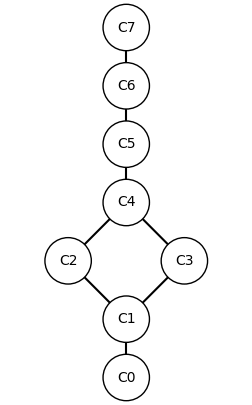
\includegraphics[scale = 0.3]{im/ex-ma2-R4.png}
	\end{minipage}
	\caption{The relations $R_3$ and $R_4$ of the contexts $\M_3$ and $\M_4$ in Example~\ref{ex:multiadjoint-bonds-2} together with the concept lattices of the contexts.}
	\label{tab:example2-multiadjoint-bonds-R3-R4}
	\vspace{-0.5cm}
\end{table}

If we look at the rows of $R_3$ and the columns of $R_4$ we can see that there is a bottom element (the number $0$) in each. Proposition~\ref{prop:trivial-multiadjoint-bonds} states that $\M_{3\,4}^\bot = (O_3, P_4, R_{3\,4}^\bot, \sigma_{3\,4})$ is a bond from $\M_3$ to $\M_4$ and $\M_{4\,3}^\bot = (O_4, P_3, R_{4\,3}^\bot, \sigma_{4\,3})$ is not a bond, for any maps $\sigma_{3\,4} \colon O_3 \times P_4 \to \{\adjoint^*_\G, \adjoint^*_\L\}$, $\sigma_{4\,3} \colon O_4 \times P_3 \to \{\adjoint^*_\G, \adjoint^*_\L\}$.

Let $\M$ be the context obtained by joining $\M_3$ and $\M_4$ with the relations $R_{3\,4}^\bot$ and $R_{4\,3}^\bot$, as in Table~\ref{tab:example2-multiadjoint-bonds-R3+R4}. If we compare its concept lattice with the third one from Fig.~\ref{fig:example1-multiadjoint-bonds-concept-lattices}, both look like the \editornote{suma disjunta de los factores}. In the latter, the concept lattice is indeed the \editornote{suma disjunta de los factores}. The concept lattice $\calC(\M)$ resembles the \editornote{suma disjunta} of $\calC(\M_3)$ and $\calC(\M_4)$, but the bottom of $\calC(\M_3)$ turns into the bottom of $\calC(\M)$ and the top of $\calC(\M_4)$ turns into the top of $\calC(\M)$.
\begin{table}
	\centering
	\vspace{-0.5cm}
	\begin{minipage}{0.3\textwidth}
	\begin{tabular}{w{c}{20pt} || w{c}{20pt} | w{c}{20pt} || w{c}{20pt} | w{c}{20pt}}
		& $a_1$ & $a_2$ & $a_3$ & $a_4$ \\\hline\hline
		$x_1$ & $0.75$ & $0$ & $0$ & $0$ \\\hline
		$x_2$ & $0.25$ & $0$ & $0$ & $0$ \\\hline\hline
		$x_3$ & $0$ & $0$ &$0$ & $0$ \\\hline
		$x_4$ & $0$ & $0$ &$0.5$ & $1$
	\end{tabular}
	\end{minipage}
	\hspace{1cm}
	\begin{minipage}{0.3\textwidth}
	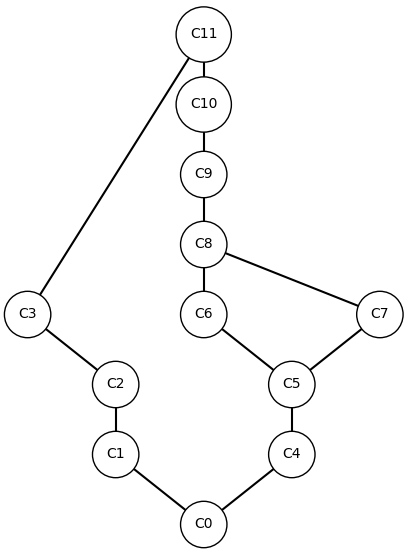
\includegraphics[height = 4cm]{im/ex-ma2-R3+R4.png}
	\end{minipage}
	\begin{minipage}{0.25\textwidth}
	\begin{tabular}{w{c}{25pt} || w{c}{25pt} | w{c}{25pt}}
		& $P_i$ & $P_j$ \\[3pt]\hline\hline&&\\[-7pt]
		$O_i$ & $\M_i$ & $\M_{ij}^\bot$ \\[3pt]\hline&&\\[-7pt]
		$O_j$ & $\M_{ji}^\bot$ & $\M_j$ \\[3pt]
	\end{tabular}
	\end{minipage}
	\caption{On the left, the relation of the context $\M$ in Example~\ref{ex:multiadjoint-bonds-2} constructed by placing the relation $R_3$ in the top left, the relation $R_{3\,4}^\bot$ in the top right, the relation $R_{4\,3}^\bot$ in the bottom left and the relation $R_4$ in the bottom right. On the center, its concept lattice. On the right, a general way of constructing the matrix $\M$ for arbitrary contexts $\M_i$ and $\M_j$.}
	\label{tab:example2-multiadjoint-bonds-R3+R4}
	\vspace{-0.5cm}
\end{table}

This is the case in general. Let $\M_i$ and $\M_j$ be two different contexts, and let $\M$\editorcomment{introduce some notation? Like $\M_1 \obot \M_2$ or $\M_1 \cupbot \M_2$. De esta forma no reutilizariamos el nombre $\M$ que he usado en el párrafo anterior.} be the context constructed from $\M_i$, $\M_j$, $\M_{ij}^\bot$ and $\M_{ji^\bot}$, as illustrated in Table~\ref{tab:example2-multiadjoint-bonds-R3+R4}. Then, when comparing the concept lattices $\calC(\M_i)$, $\calC(\M_j)$ and $\calC(\M)$, if the bottom element of $\calC(\M_i)$ turns into the bottom element of $\calC(\M)$ and if the top element of $\calC(\M_j)$ turns into the top element of $\calC(\M)$, then the context $\M_{ij}^\bot$ is a bond from $\M_i$ to $\M_j$. Dually, if the bottom element of $\calC(\M_j)$ turns into the bottom element of $\calC(\M)$ and if the top element of $\calC(\M_i)$ turns into the top element of $\calC(\M)$, then the context $\M_{ji}^\bot$ is a bond from $\M_j$ to $\M_i$. It is possible to have both simultaneously, which means that both $\M_{ij}^\bot$ and $\M_{ji}^\bot$ are bonds.

A few examples of this are presented in Figure~\ref{fig:example2-multiadjoint-bonds-concept-lattices}. For the first one, $\M_{ij}^\bot$ is a bond from $\M_i$ to $\M_j$ and also $\M_{ji}^\bot$ is a bond from $\M_j$ to $\M_j$. For the second one, $\M_{ji}^\bot$ is a bond from $\M_j$ to $\M_j=i$ but $\M_{ij}^\bot$ is not a bond from $\M_i$ to $\M_j$.

\begin{figure}
	\begin{minipage}{\textwidth}
		\begin{minipage}{0.35\textwidth}
			\centering
			\begin{tabular}{w{c}{20pt} || w{c}{20pt} | w{c}{20pt} || w{c}{20pt} | w{c}{20pt}}
				& $a_1$ & $a_2$ & $a_3$ & $a_4$ \\\hline\hline
				$x_1$ & $0.75$ & $0$ & $0$ & $0$ \\\hline
				$x_2$ & $0$ & $0$ & $0$ & $0$ \\\hline\hline
				$x_3$ & $0$ & $0$ & $0$ & $0.25$ \\\hline
				$x_4$ & $0$ & $0$ & $0.25$ & $0$
			\end{tabular}
		\end{minipage}
		\hspace{1cm}
		\begin{minipage}{0.1\textwidth}
			\centering
			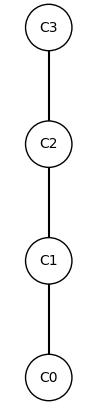
\includegraphics[height = 2\textwidth]{im/ex-ma2-other-contexts-1.png}
		\end{minipage}
		\begin{minipage}{0.2\textwidth}
			\centering
			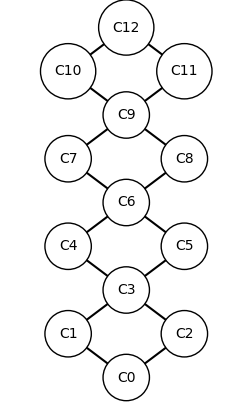
\includegraphics[height = \textwidth]{im/ex-ma2-other-contexts-2.png}
		\end{minipage}
		\begin{minipage}{0.2\textwidth}
			\centering
			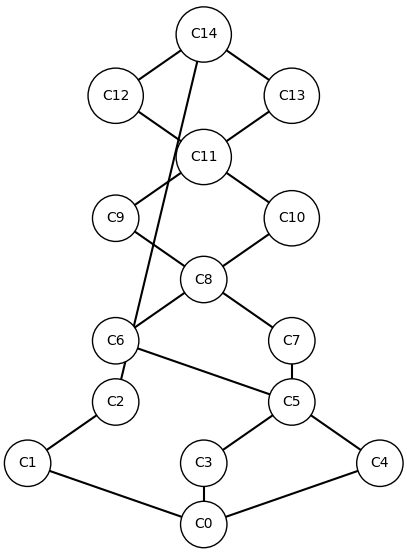
\includegraphics[height = \textwidth]{im/ex-ma2-other-contexts-1+2.png}
		\end{minipage}
	\end{minipage}

	\vspace{0.3cm}
	\begin{minipage}{\textwidth}
		\begin{minipage}{0.35\textwidth}
			\centering
			\begin{tabular}{w{c}{20pt} || w{c}{20pt} | w{c}{20pt} || w{c}{20pt} | w{c}{20pt}}
				& $a_1$ & $a_2$ & $a_3$ & $a_4$ \\\hline\hline
				$x_1$ & $1$ & $0$ & $0$ & $0$ \\\hline
				$x_2$ & $0$ & $0.25$ & $0$ & $0$ \\\hline\hline
				$x_3$ & $0$ & $0$ & $0.75$ & $0$ \\\hline
				$x_4$ & $0$ & $0$ & $0.75$ & $0$
			\end{tabular}
		\end{minipage}
		\hspace{1cm}
		\begin{minipage}{0.2\textwidth}
			\centering
			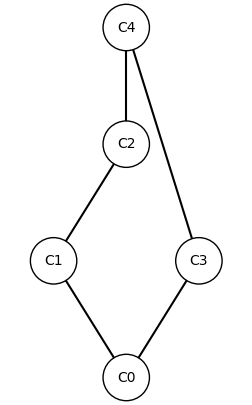
\includegraphics[height = \textwidth]{im/ex-ma2-other-contexts-3.png}
		\end{minipage}
		\begin{minipage}{0.1\textwidth}
			\centering
			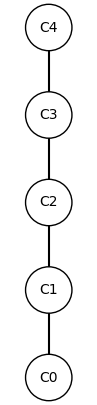
\includegraphics[height = 2\textwidth]{im/ex-ma2-other-contexts-4.png}
		\end{minipage}
		\begin{minipage}{0.2\textwidth}
			\centering
			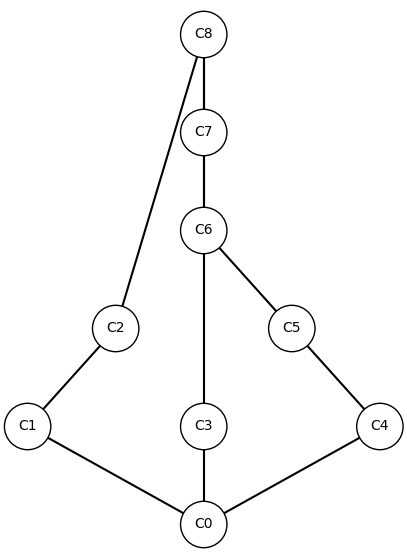
\includegraphics[height = \textwidth]{im/ex-ma2-other-contexts-3+4.png}
		\end{minipage}
	\end{minipage}
	\caption{Two examples of bonds joined together by the empty contexts as explained in Example~\ref{ex:multiadjoint-bonds-2}. On the right of each table, the concept lattice for the first context, the second context, and the full context presented in the table, in order.}
	\label{fig:example2-multiadjoint-bonds-concept-lattices}
\end{figure}

\end{example}

\section{Conclusions and future work}

%\section*{References}

%\bibliographystyle{plain}
%\bibliography{GlobalBibliography}

{\small
\bibliographystyle{abbrv}
\bibliography{conceptLattice,fuzzyLP}
}



\end{document}
